An example CF-QCM response for free particles is depicted to the left in
\Figure{fig:expsetup}(b).  Here, free \SI{1}{\micro\meter} streptavidin
coated polystyrene particles in water are introduced into the sample cell.
When the cell is rotated to the loading configuration under the influence
of gravity alone, the particles fall toward the sensing surface and a positive
shift in the QCM's frequency signal is observed.  When the cell is then
rotated 180 degrees to the unloading configuration, the particles fall off
and the frequency response returns to its original state.  Again the cell
is rotated 180 degrees to the loading configuration and the positive
frequency shift is observed.  As the centrifuge spins up towards
\SI{90}{g}, the particles are ``pressed'' towards the QCM surface and a
four fold increase in the frequency shift is observed.  The centrifuge then
spins down and the baseline frequency shift under gravity alone is
recovered.

Traditional QCM experiments assume that the inertial properties and
rigidity of the sample's coupling are taken as a fixed parameter (or
statistical distribution) under assay.  With this approach however, one is
only able to obtain discrete values in an otherwise continuous parameter space.  Hybrid-QCM experiments
involving nanoindenters~\cite{borovsky2001measuring} or AFM probe
tips~\cite{richter2003pathways} have shown intriguing behavior when force
is applied to a sample in a QCM measurement.  There have also been reports
that accelerations as small as \SI{1}{g} have a measurable effect on a
QCM's response for viscoelastic monolayers such as
DNA~\cite{fawcett2004evidence}, and even for pure Newtonian
liquids~\cite{yoshimoto2002effect}.  All of these responses have been found
to be significant compared to the baseline acceleration sensitivity of the
QCM itself~\cite{filler1988acceleration}.  With the integration of a
centrifuge to a standard QCM, one can observe these effects under enhanced
g-forces and make endpoint measurements (measurements taken after the
addition of a sample) in the sample's parameter space continuously and
repeatedly.

To demonstrate this, we have examined six different samples in the CF-QCM
under variable accelerations from approximately \SIrange{1}{90}{g}.  These
samples were chosen to be examples of the breadth of load situations
accessible with our technique.  They are:
\begin{inparaenum}[(a)]
\item air,
\item deionized water,
\item free particles in water,
\item paramagnetic particles attached to the sensor via short oligonucleotides,
\item \SI{48}{kbp} lambda phage DNAs attached to the gold electrode, and
\item polystyrene particles tethered to the sensor via \SI{48}{kbp} lambda phage DNAs.
\end{inparaenum}

The employed QCM driver circuit outputs Butterworth van Dyke (BvD)
equivalent relative frequency $\df$ (in hertz) and motional resistance $R$ (in ohms).
$R$ is approximately related to the bandwidth $\Gamma$ (half width at half
maximum of the frequency response) by $\Gamma=R/\left(4\pi L\right)$, where
$L=\SI{40}{\milli\henry}$ is the motional inductance of the BvD
equivalent circuit~\cite{arnau2002circuit}.  For this
relationship we assume the small load approximation $\df/f_\mathrm{F} \ll
1$, where $f_\mathrm{F}$ is the fundamental frequency~\cite{geelhood2002transient}.
It is therefore relevant to note our assumption that $\Delta R$ is an
approximate, and indirect, measure of the bandwidth $\dg$ (in
hertz).  In addition $\dg$ is an equivalent representation of the ``dissipation'', $D$, used in
QCM-D devices by $D=2\dg/f_\mathrm{F}$ 
\begin{figure*}[ht]
\centering
%\hspace{-1.0cm}
%\includegraphics{Figure-3_webster.pdf}
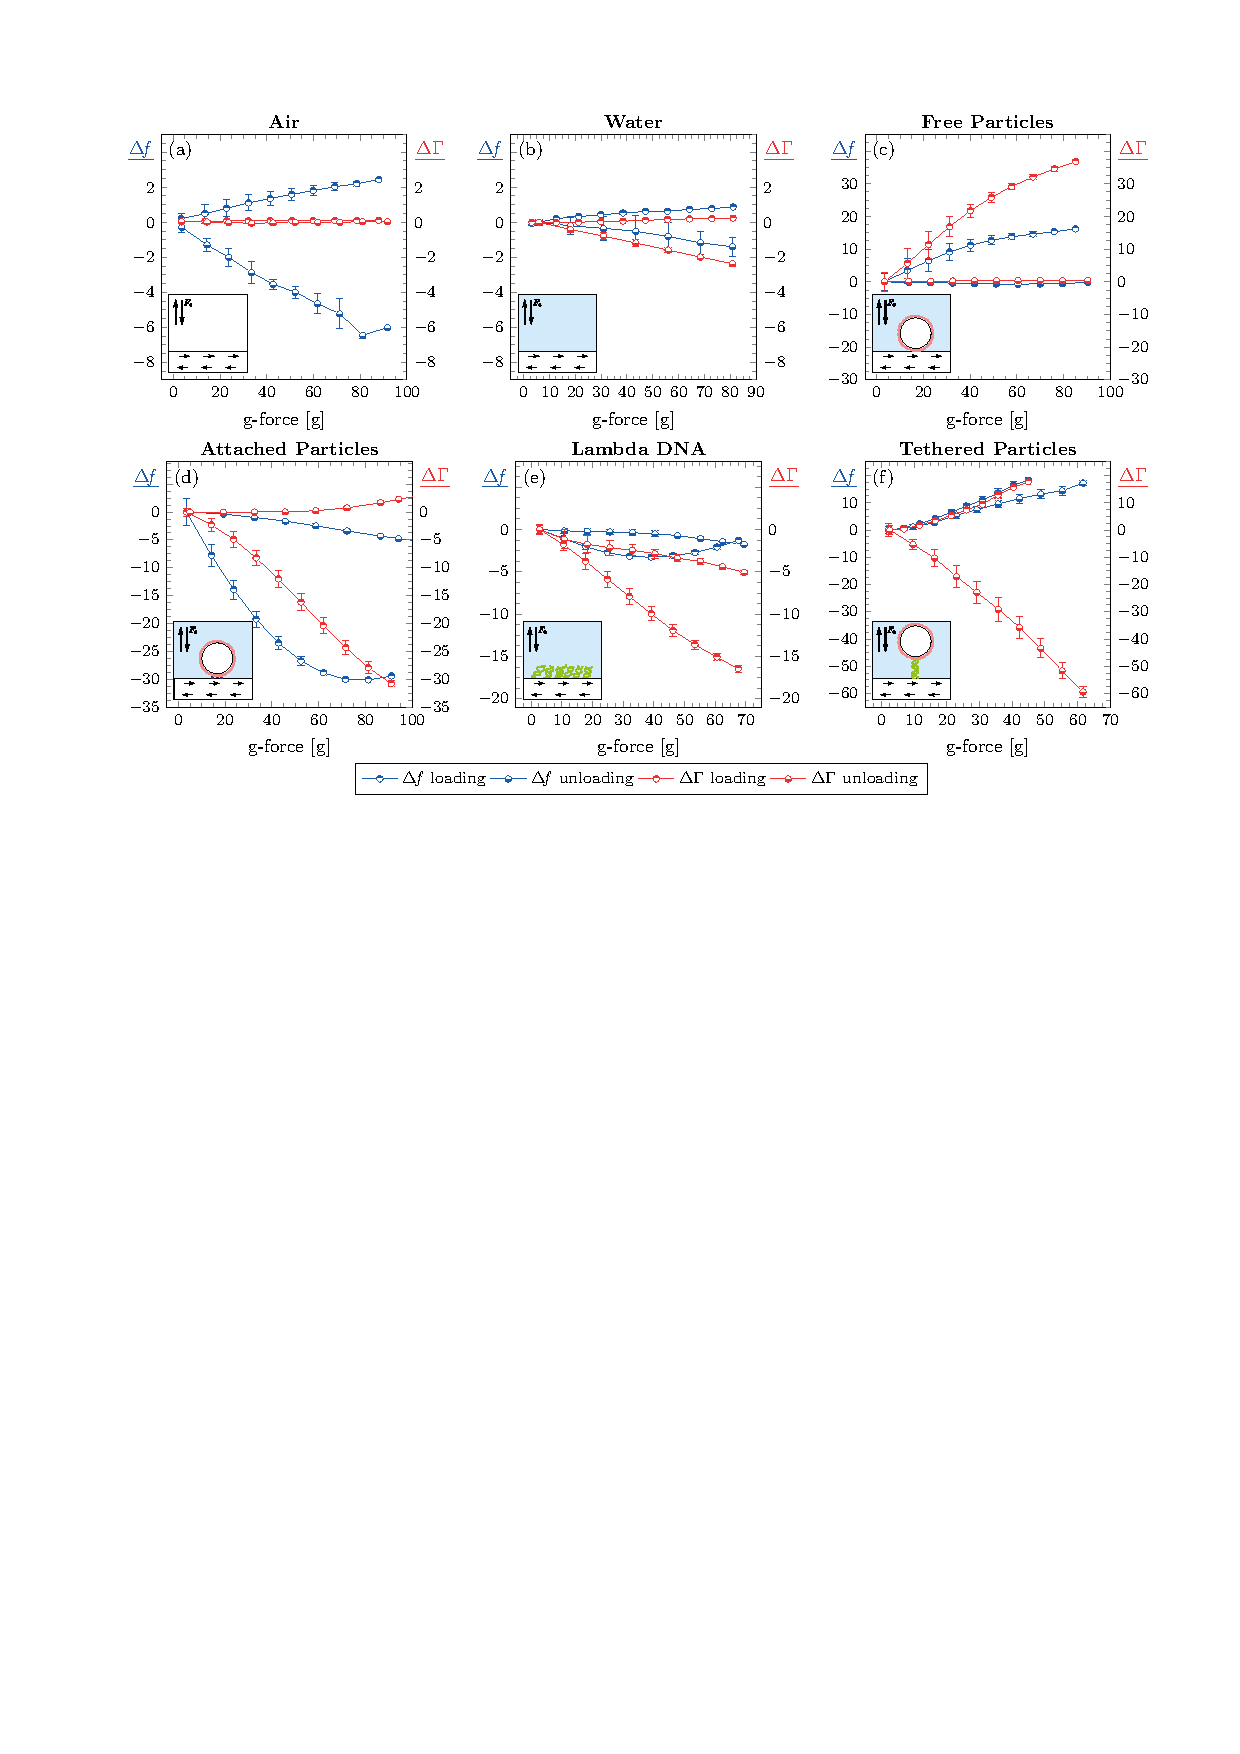
\includegraphics{qcm/figures/figure2.pdf}
\caption{Load situations.
Change in frequency $\df$ and bandwidth $\dg$
(in hertz, inferred from motional resistance) of
the CF-QCM under different load situations as the centripetal acceleration
is directed in to (\textit{loading}, represented by circles with the top half
colored) and out of (\textit{unloading}, represented by circles with the
bottom half colored) the plane of the crystal.
The situations are 
(a) unloaded crystal in air, 
(b) deionized water, 
(c) free \SI{1}{\micro\meter} diameter streptavidin coated polystyrene
particles, $N_\mathrm{L}=\SI{1.58e11}{\particle\per\meter\squared}$,
(d) \SI{2}{\micro\meter} diameter streptavidin coated paramagnetic
particles, $N_\mathrm{L}=\SI{1.65e10}{\particle\per\meter\squared}$,
attached with \SI{25}{mer} oligonucleotides, 
(e) lambda DNA only attached to the gold electrode, and
(f) \SI{25}{\micro\meter} diameter streptavidin
coated polystyrene particles,
$N_\mathrm{L}=\SI{3.25e7}{\particle\per\meter\squared}$, tethered to the sensor surface with
\SI{48}{kbp} lambda DNAs.  Error bars are derived from uncertainties
(standard deviation) in
the centrifuge both spinning up and spinning down in a single experimental
run.
} 
\label{fig:loadplot}
\end{figure*}

\section{Air}
The instrument's response was first tested in air, shown in
\Figure{fig:loadplot}(a).  The base acceleration sensitivity (change in
frequency versus change in g-force) of AT cut quartz normal to the plane of
the crystal has a reported value~\cite{valdois2794influence} of $\df/\Delta
g =\SI{2.188+-0.006e-2}{\hertz\per\g}$.  Our instrument shows similar
behavior: $\df/\Delta g =\SI{2.682+-0.023e-2}{\hertz\per\g}$ in the loading
configuration.  The signs of $\df/\Delta g$ are found to be opposite in the
loading and unloading configurations.  We have not found a reference for
the bandwidth or motional resistance dependence of a QCM under
acceleration, but we find the value to be $\dg/\Delta g =
\SI{9.203+-0.171e-4}{\hertz\per\g}$.

\section{Deionized Water}
Next, deionized water was used as a control sample for measurement in the
liquid phase, as shown in \Figure{fig:loadplot}(b).  The initial shift in
frequency and bandwidth is in agreement with what is obtained the Kanazawa-Gordon
relations~\cite{kanazawa1985frequency} for water
($\rho=\SI{1}{\gram\per\centi\meter\cubed}$ and
$\eta=\SI{1}{\milli\pascal\second}$): $\df = \SI{-714}{\hertz}$ and
$R=\SI{359}{\ohm}$, which are close to the measured values of $\df =
\SI{-716}{\hertz}$ and $R=\SI{357}{\ohm}$.  The response under centrifugal
load was found to be linear and smaller than that of air: $\df/\Delta g=
\SI{1.357+-0.024e-2}{\hertz \per\g}$ and $\dg/\Delta g=
\SI{2.865+-0.073e-3}{\hertz\per\g}$.  We observe that these acceleration
dependent forces in the liquid phase are not necessarily commensurate with
those in the gas phase, but as the effects are small compared to
experiments with actual loads, we treat them as baselines to be
subtracted.

\section{Free Particles}
Utilizing the flexibility that the instrument provides in modifying the
coupling between the load and the sensor surface, we have applied the
technique to the study of discrete micron sized particles.  As first
referenced in \Figure{fig:expsetup}(b), the frequency and bandwidth shifts
of free particles in the liquid phase as a function of g-force is shown in
\Figure{fig:loadplot}(c).  Here, streptavidin coated polystyrene particles,
mean diameter $\bar{d}=\SI{1.07}{\micro\meter}$, are placed in the sample volume with
a surface density of
$N_\mathrm{L}=\SI{1.58e11}{\particle\per\meter\squared}$ and the signal is
observed in both the loading and unloading configurations.
The particles
did not exhibit adhesion to either the unmodified gold electrode or the
glass/PDMS cell surrounding it; in the unloading configuration, the particles
quickly drifted away from the sensing area and a signal identical to water
was observed.  In the loading configuration, a large positive
shift in $\df$ and $\dg$ was observed, consistent with
previously observed responses for weakly coupled particles in this size
range~\cite{johannsman2007contacts}.  

The initial shift under \SI{1}{g} was found to be $\df=
\SI{2.2}{\hertz}$ and $\dg=\SI{7.5}{\hertz}$.  At the maximum acceleration of \SI{90}{g} the
signal increases to $\df = \SI{16.5}{\hertz}$ and $\dg=\SI{37}{\hertz}$. This also
represents a sensitivity enhancement in the minimum resolvable surface
density of the particles.  The scaling of $\df$ and $\dg$ with increasing
centrifugal load is nonlinear in the applied load, implying non-Hertzian
behavior~\cite{borovsky2001measuring}.
%The exact mechanism of coupling and relation of the applied force with is
%beyond the scope of this manuscript.

The same experiment was also carried out with \num{2}, \num{6}, \num{15},
and \SI{25}{\micro\meter} polystyrene particles.
%(actual mean diameters $d=\bar{d}=1.89, 5.86,, 15\,\mathrm{and}\;\SI{24.8}{\micro\meter}$).
The loading curves all
followed the same trend, but the relative shifts in $\df$ and $\dg$
differed based on particle size.  The results from these loads
are summarized in \Table{tbl:particlesize}.
\begin{table}[h]
 \centering
	Frequency and Bandwidth Shifts\\
 \begin{tabularx}{240pt}{XXXXX}
 \toprule
 $\bar{d}$ [\si{\micro\meter}] & $\df_1/N_\mathrm{L}$ & $\dg_1/N_\mathrm{L}$ & $\df_{90}/N_\mathrm{L}$ & $\dg_{90}/N_\mathrm{L}$ \\
 \midrule
 %cat table.txt | sed -e s/E-/\\\\text{\\\\sc{e}-}/g | sed -e ``s/\t/ \& /g''
$1.07^p$ & 1.61\text{\sc{e}-}11 & 3.85\text{\sc{e}-}11 & 6.98\text{\sc{e}-}11 & 1.43\text{\sc{e}-}10\\
$1.89^m$ & 5.58\text{\sc{e}-}11 & 6.55\text{\sc{e}-}11 & 7.90\text{\sc{e}-}10 & 2.43\text{\sc{e}-}10\\
$5.86^m$ & 4.00\text{\sc{e}-}09 & 3.09\text{\sc{e}-}09 & 3.43\text{\sc{e}-}10 & 3.41\text{\sc{e}-}10\\
$15.0^p$ & 1.32\text{\sc{e}-}07 & 6.39\text{\sc{e}-}08 & 3.99\text{\sc{e}-}08 & 9.50\text{\sc{e}-}09\\
$24.80^p$ & 5.01\text{\sc{e}-}07 & 1.53\text{\sc{e}-}07 & 3.26\text{\sc{e}-}07 & 1.65\text{\sc{e}-}07\\
 \bottomrule
\end{tabularx}
\caption{Normalized frequency and bandwidth shifts (in
 \si{\hertz\meter\squared} at \num{1} and
\SI{90}{g} for various particle sizes in water. The quoted diameter
$\bar{d}$ is
their mean diameter. $p$: polystyrene particles, $m$:
magnetite coated polystyrene.}
\label{tbl:particlesize}
\end{table}

\section{Oligo Attached Particles}
In contrast to the situation of free particles, we have also studied the
behavior of the CF-QCM in a regime where particles are rigidly coupled to
the sensor by attaching \SI{2}{\micro\meter} (mean diameter
$\bar{d}=\SI{1.89}{\micro\meter}$) streptavidin coated paramagnetic
particles modified with biotinylated \SI{25}{mer} oligos to complimentary
strands conjugated to the QCM gold surface via thiol bonds (see
Materials).  This is shown in \Figure{fig:loadplot}(d).  Note
that, $\df$ and $\dg$ are both negative and decrease
with centrifugal force in the loading orientation.  
When spinning with the oligo attached
particles, we suspect we are not sensing the presence of the particle
directly but rather the conformational state of the oligonucleotide layer.
Such an acceleration effect has been observed
before~\cite{yoshimoto2002effect}~\cite{fawcett2004evidence}, but only
within the \SI{2}{g} orientation difference of gravity.  When the oligo
layer is under centrifugal load, it compresses, causing the
density-viscosity product to increase.  This behavior is consistent with
the behavior of DNA observed on QCMs under the influence of gravity
alone~\cite{fawcett2004evidence}.
%The initial trend in
%frequency follows Sauerbrey (negative frequency shift proportional to mass
%adsorption) like behavior.  For mass loading at this number density, the
%predicted frequency shift is  $\SI{-0.49}{\hertz}$.  At \SI{95}{g}
%$\df = \SI{-30}{\hertz}$, which approximately follows a linear
%increase of inertial mass.  
%We observe a \SI{5}{\percent} change in this product at \SI{90}{g}.  

\section{Lambda DNA}
Moving from particles to viscoelastic monolayers, in
\Figure{fig:loadplot}(e), \SI{48}{kbp} lambda phage DNA in STE buffer were
attached to the gold sensor electrode via a complimentary thiolated oligo.  Previous studies have shown that,
through the use of dissipation monitoring, QCMs are sensitive to not only
the adsorbed mass and viscosity, but the physical conformal state
(``shape'') of DNAs hybridized to the sensor
surface~\cite{tsortos2008shear}.  In the experiment, even though the force
on the lambda DNAs is on the order of femtonewtons, we observe a strong
linear decrease ($\dg=\SI{-2.912+-0.0095}{\hertz\per\g}$) in the
bandwidth as function of g-force, indicating an
increase in viscoelastic loss.  However, under larger g-forces the sign of
$\df$ reverses.  The origin of this effect is not understood, but
could indicate a nonlinear viscoelastic compliance under load.  The
unloading configuration sees a smaller negative response in $\dg$ with little
effect on $\df$.

At this point we make an observation about the influence of salt buffer,
which was used in experiments involving DNA.  There are several
studies~\cite{encarnaccao2007influence}~\cite{lin1995role} regarding the
effects of various electrolytic buffer solutions and their concentrations
on QCM measurements, including reports of an immersion angle (and therefore
gravity) dependence~\cite{yoshimoto2006characteristics}.  These reports
suggest this effect may be related to the behavior of the interfacial layer
and ion transport in monovalent electrolytic solutions in accelerating
frames~\cite{tolman1911electromotive}~\cite{des1893unpolarisirbare}.  We
have observed a significant contribution in the unloading configuration for
STE buffer alone ($\df=\SI{-0.326+-0.0029}{\hertz\per\g}$, and $\dg$
nonlinear), which was subsequently ``screened''~\cite{zhang2002insulating}
by the presence of both oligos and lambda DNAs, making the effect
negligible in the current set of experiments.  Further investigation is
required to explain this precisely.

\section{Tethered Particles}
With the sensitivity to both particles and monolayers, the instrument
raises a possibility for using beads tethered by lambda DNA as a
transduction mechanism to investigate its kinetics.  One such example is
shown in \Figure{fig:loadplot}(f).  Streptavidin coated polystyrene
particles with a mean diameter of \SI{24.8}{\micro\meter} were tethered to
the CF-QCM by means of a \SI{48}{kbp} lambda phage DNA.  Experiments were
done in STE buffer whose density reduced the maximum force the bead could
exert to about \SI{40}{\pico\newton} which, according to the worm-like
chain model~\cite{marko1995stretching}, should almost fully extend the
lambda DNA to a length of \SI{16}{\micro\meter}.

Though the instrument has not yet been developed enough to make accurate
quantitative measurements in this load situation, the behavior of the data
is a clear indication of its potential.  As the tethered bead extends the
DNA under centrifugal force, $\df$ increases and $\dg$ decreases.  In the
case where the DNAs are trapped and pushed between the bead and the
surface, both $\df$ and $\dg$ increase.  We have confirmed the signs of the
shifts in this scenario with \SI{10}{\micro\meter} and \SI{6}{\micro\meter}
paramagnetic particles, using a magnet to either pull or push the
particles toward or away from the sensor surface.  This behavior is
distinct from either the case of lambda DNA or free particles alone.

At $F_\mathrm{c}=\SI{40}{\pico\newton}$, the frequency shift indicates an
effective decrease in the density-viscosity product of \SI{10}{\percent} or
about \SI{1.5}{\pico\gram}.  For the surface densities involved
($N_\mathrm{L}=\SI{3.25e7}{\particle\per\meter\squared}$), the equivalent
interfacial mass lost for a fully extended lambda DNA predicted by the
worm-like chain model are in the picogram range and cannot account for the
more than $10^6$ signal difference shown here.  If indeed the response is
due to lambda DNA extension, future experiments involving high frequency,
large centrifugal force CF-QCMs could easily detect the kinetics of a
single tether.

\section{Particle Sizing}
\begin{figure}[ht]
\centering
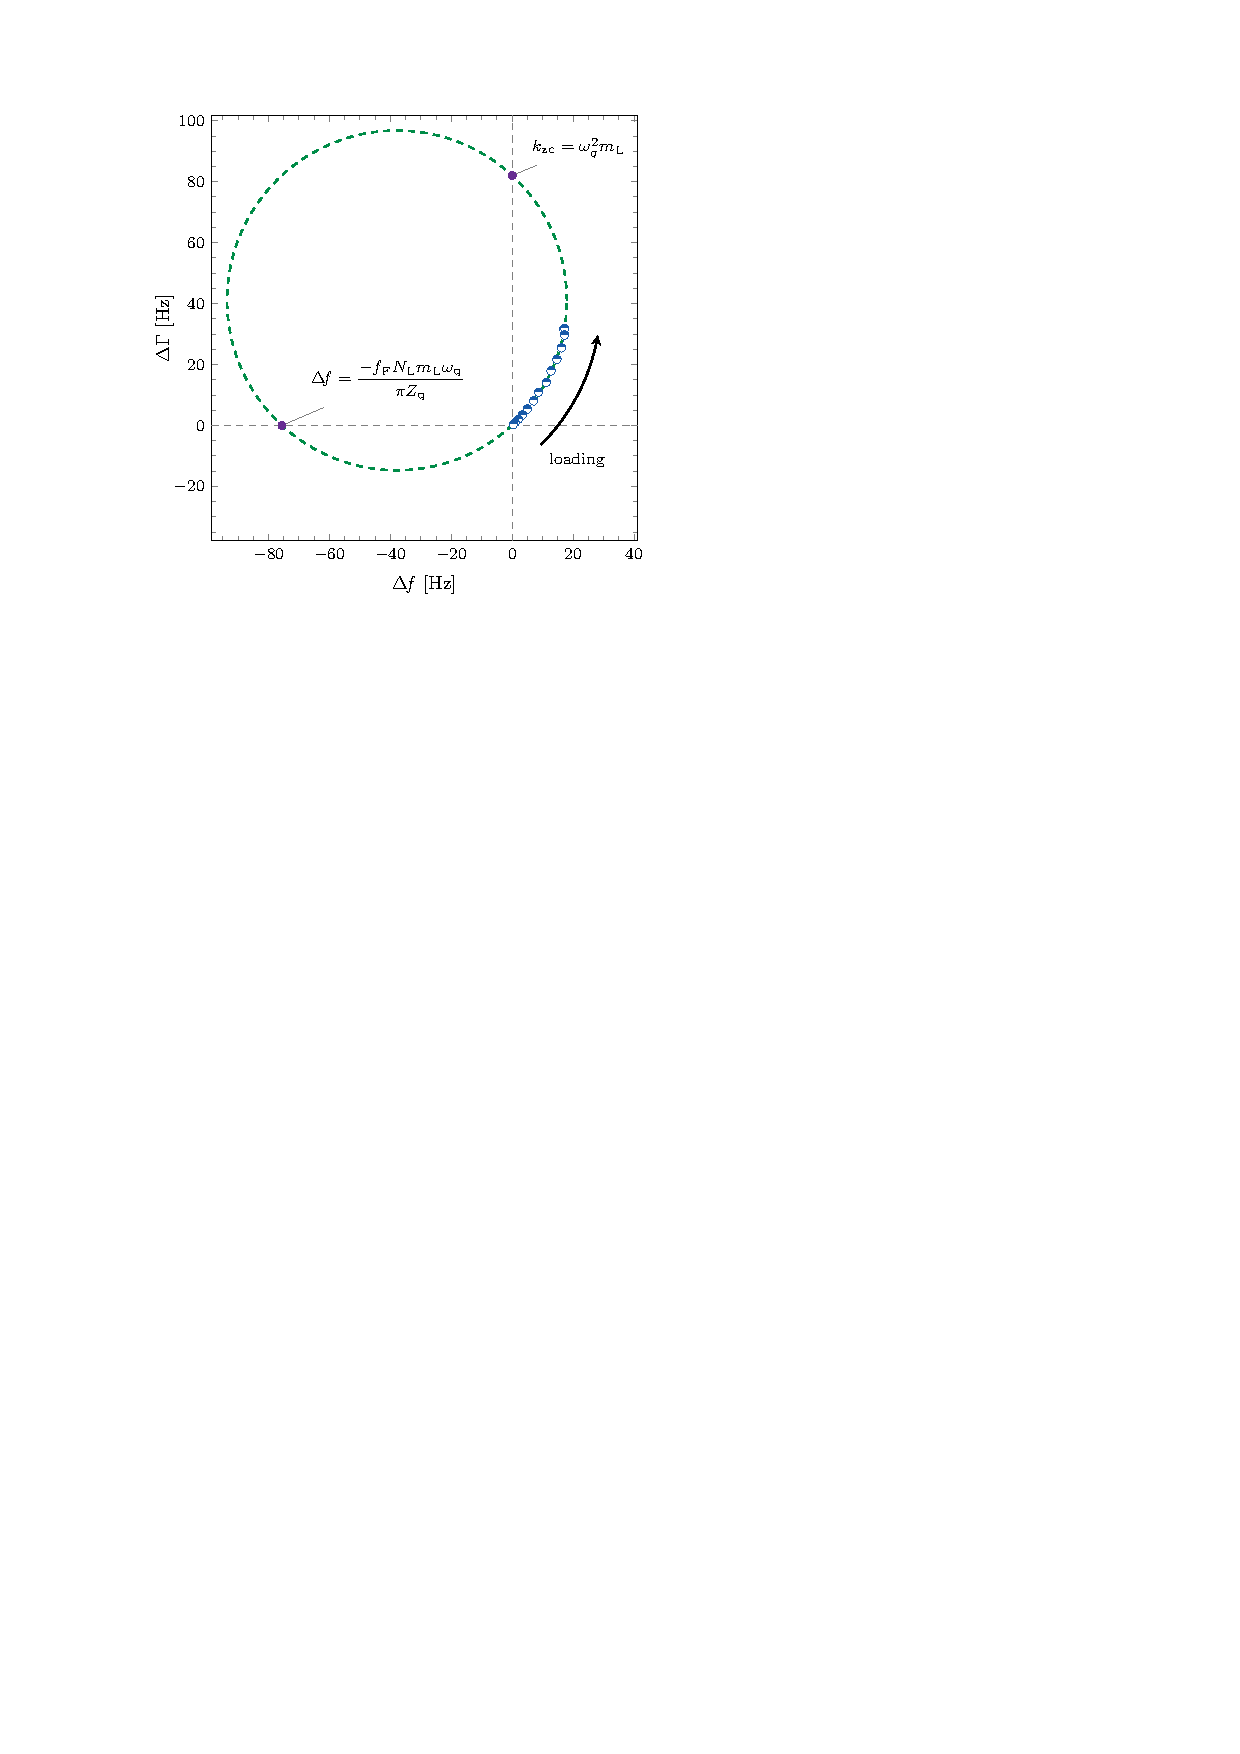
\includegraphics{qcm/figures/figure4.pdf}
\caption{ Particle sizing.  Method for sizing micron-sized particles using the CF-QCM. 
$\df$ versus $\dg$ is plotted parametrically as a function of g-force, and
the data is fit to a circle.  The point on the circle for which $\dg=0$ and
$\df<0$ provides an estimate of mass adsorption, and thus particle size.
Results for particles with diameters $\bar{d}_\mathrm{actual}=1, 2,
15,\,\mathrm{and}\;\SI{25}{\micro\meter}$ are shown in
\Table{tbl:particlesizing}.  Fit circle has a radius of \SI{55.77}{\hertz} and
a center of $(-37.83,41.05) \si{\hertz}$. }
\label{fig:circlefit}
\end{figure}

The coupled oscillator model (\Equation{eqn:mastereq}), when analyzed for
samples of free particles (\Figure{fig:expsetup}(b),
\Figure{fig:loadplot}(c), and \Table{tbl:particlesize}), suggests an avenue
to allow QCMs to determine the size of large micron-sized particles in the
liquid phase.  Thus far this has only been possible with nanometer-sized
particles which lie within the QCM's shear acoustic
wave.~\cite{olsson2013using}  If one plots $\df$ verses $\dg$ in
\Equation{eqn:mastereq} as a parametric function of $\kl$, the points are
found to lie on a circle with radius $r_\mathrm{L}$.  In doing so, the physical
mechanism modifying $\kl$ is removed from the problem.
If we then fit a
circle to the experimentally observed $\df$-$\dg$ data (plotted
parametrically as a function of g-force), we can extrapolate the behavior
in the strong coupling regime by finding the point at which $\dg=0$ and
$\df<0$.  Knowing $\df$, \Equation{eqn:couplinguy2} can then be inverted to
solve for either number density or particle size/mass.  An example of this
procedure is shown in \Figure{fig:circlefit} using the same data for
\SI{1}{\micro\meter} particles shown in
\Figure{fig:expsetup} and \Figure{fig:loadplot}.  Inset is a table for the same
predictions done for particles with known diameter
$\bar{d}_\mathrm{actual}=1, 2, 15,\,\mathrm{and}\;\SI{25}{\micro\meter}$.
In all cases the surface density was known and the diameter
$\bar{d}_\text{predicted}$ was derived from the mass $\ml$, found by
inverting \Equation{eqn:couplinguy2}.  The results are surprisingly accurate
despite the exploratory nature of the instrument's construction, which
illustrates the robustness of this unique methodology that CF-QCM
provides.
It should also be mentioned that with knowledge of the way in which the
g-force modifies $\kl$, the frequency zero crossing at
$k_\mathrm{zc}=\omegaq^2\ml$ can be used to determine the mass $\ml$
without knowledge of the number density $N_\mathrm{L}$. 
\begin{table}[ht]
\centering
Particle Sizing\\
 \begin{tabularx}{80pt}{XX}
 \toprule
 $\bar{d}_\mathrm{actual}$ & $\bar{d}_\mathrm{predicted}$ \\
 \midrule
  $1.07^p$ & \num{1.23+-0.23} \\
  $1.89^m$ & \num{1.84+-0.06} \\
  $15.0^p$ & \num{13.8+-1.3} \\
  $24.8^p$ & \num{22.6+-4.6} \\
 \bottomrule
\end{tabularx}
\caption{Results of the particle sizing method applied to particles with diameters
$\bar{d}_\mathrm{actual}=1, 2, 15,\,\mathrm{and}\;\SI{25}{\micro\meter}$.}
\label{tbl:particlesizing}
\end{table}

\section{Strange Buffer Effects}

\begin{itemize}
\item Temperature effects as described in the manual are most accurate,
but are too slow compared to the force-frequency curves we see.
\item Pressure is also ruled out. The mass difference between water and
\SI{1}{M} \ce{NaCl} is about \SI{7.5}{\milli\gram}, while the signal
difference is \SI{-1}{\hertz} for water and \SI{-30}{\hertz} for
\SI{1}{M} \ce{NaCl}.
\item Mechanical stress also ruled out for the same reason.
\end{itemize}
